%%%%%%%% ICML 2023 EXAMPLE LATEX SUBMISSION FILE %%%%%%%%%%%%%%%%%

\documentclass{article}

% Recommended, but optional, packages for figures and better typesetting:
\usepackage{microtype}
\usepackage{graphicx}
\usepackage{subfigure}
\usepackage{booktabs} % for professional tables

\usepackage{tikz}
% Corporate Design of the University of Tübingen
% Primary Colors
\definecolor{TUred}{RGB}{165,30,55}
\definecolor{TUgold}{RGB}{180,160,105}
\definecolor{TUdark}{RGB}{50,65,75}
\definecolor{TUgray}{RGB}{175,179,183}

% Secondary Colors
\definecolor{TUdarkblue}{RGB}{65,90,140}
\definecolor{TUblue}{RGB}{0,105,170}
\definecolor{TUlightblue}{RGB}{80,170,200}
\definecolor{TUlightgreen}{RGB}{130,185,160}
\definecolor{TUgreen}{RGB}{125,165,75}
\definecolor{TUdarkgreen}{RGB}{50,110,30}
\definecolor{TUocre}{RGB}{200,80,60}
\definecolor{TUviolet}{RGB}{175,110,150}
\definecolor{TUmauve}{RGB}{180,160,150}
\definecolor{TUbeige}{RGB}{215,180,105}
\definecolor{TUorange}{RGB}{210,150,0}
\definecolor{TUbrown}{RGB}{145,105,70}

% hyperref makes hyperlinks in the resulting PDF.
% If your build breaks (sometimes temporarily if a hyperlink spans a page)
% please comment out the following usepackage line and replace
% \usepackage{icml2023} with \usepackage[nohyperref]{icml2023} above.
\usepackage{hyperref}


% Attempt to make hyperref and algorithmic work together better:
\newcommand{\theHalgorithm}{\arabic{algorithm}}

\usepackage[accepted]{icml2023}

% For theorems and such
\usepackage{amsmath}
\usepackage{amssymb}
\usepackage{mathtools}
\usepackage{amsthm}

% if you use cleveref..
\usepackage[capitalize,noabbrev]{cleveref}

%%%%%%%%%%%%%%%%%%%%%%%%%%%%%%%%
% THEOREMS
%%%%%%%%%%%%%%%%%%%%%%%%%%%%%%%%
\theoremstyle{plain}
\newtheorem{theorem}{Theorem}[section]
\newtheorem{proposition}[theorem]{Proposition}
\newtheorem{lemma}[theorem]{Lemma}
\newtheorem{corollary}[theorem]{Corollary}
\theoremstyle{definition}
\newtheorem{definition}[theorem]{Definition}
\newtheorem{assumption}[theorem]{Assumption}
\theoremstyle{remark}
\newtheorem{remark}[theorem]{Remark}

% Todonotes is useful during development; simply uncomment the next line
%    and comment out the line below the next line to turn off comments
%\usepackage[disable,textsize=tiny]{todonotes}
\usepackage[textsize=tiny]{todonotes}


% The \icmltitle you define below is probably too long as a header.
% Therefore, a short form for the running title is supplied here:
\icmltitlerunning{Project Report Template for Data Literacy 2023/24}

\begin{document}

\twocolumn[
\icmltitle{Heart of the Matter:\\A Deep Dive into Germany's Battle with Cardiovascular Diseases}

% It is OKAY to include author information, even for blind
% submissions: the style file will automatically remove it for you
% unless you've provided the [accepted] option to the icml2023
% package.

% List of affiliations: The first argument should be a (short)
% identifier you will use later to specify author affiliations
% Academic affiliations should list Department, University, City, Region, Country
% Industry affiliations should list Company, City, Region, Country

% You can specify symbols, otherwise they are numbered in order.
% Ideally, you should not use this facility. Affiliations will be numbered
% in order of appearance and this is the preferred way.
\icmlsetsymbol{equal}{*}

\begin{icmlauthorlist}
\icmlauthor{Vojtěch Sýkora}{equal,first}
\icmlauthor{Denis Kovačević}{equal,second}
\icmlauthor{Nam Nguyen The}{equal,third}
\end{icmlauthorlist}

% fill in your matrikelnummer, email address, degree, for each group member
\icmlaffiliation{first}{Matrikelnummer 6636502, vojtech.sykora@student.uni-tuebingen.de, MSc Machine Learning}
\icmlaffiliation{second}{Matrikelnummer 6707752, denis.kovacevic@student.uni-tuebingen.de, MSc Machine Learning}
\icmlaffiliation{third}{Matrikelnummer 6608479, nam.nguyen-the@student.uni-tuebingen.de, MSc Machine Learning}

% You may provide any keywords that you
% find helpful for describing your paper; these are used to populate
% the "keywords" metadata in the PDF but will not be shown in the document
\icmlkeywords{Machine Learning, ICML}

\vskip 0.3in
]

% this must go after the closing bracket ] following \twocolumn[ ...

% This command actually creates the footnote in the first column
% listing the affiliations and the copyright notice.
% The command takes one argument, which is text to display at the start of the footnote.
% The \icmlEqualContribution command is standard text for equal contribution.
% Remove it (just {}) if you do not need this facility.

%\printAffiliationsAndNotice{}  % leave blank if no need to mention equal contribution
\printAffiliationsAndNotice{\icmlEqualContribution} % otherwise use the standard text.

\begin{abstract}
    % Abstracts typically start with a sentence motivating why the subject is interesting.
    Even though modern medicine is able to overcome many obstacles in improving life quality. 
    However, without a healthy lifestyle, even the best health system are of little help. 
    In this paper, we will analyse the most prevalent health concerns in Germany and their development over time.
    We will do so by using data from multiple sources, including the Global Burden of Disease and the World Development Indicators.
    Using multivariate linear regression, we are able to identify the most important factors that influence the health of the German population.
\end{abstract}

\section{Introduction}\label{sec:intro}
Motivate the problem, situation or topic you decided to work on. Describe why it matters (is it of societal, economic, scientific value?). Outline the rest of the paper (use references, e.g.~to \Cref{sec:methods}: What kind of data you are working with, how you analyse it, and what kind of conclusion you reached. The point of the introduction is to make the reader want to read the rest of the paper.


\section{Data and Methods}\label{sec:methods}
In this section, describe \emph{what you did}. Roughly speaking, explain what data you worked with, how or from where it was collected, it's structure and size. Explain your analysis, and any specific choices you made in it. Depending on the nature of your project, you may focus more or less on certain aspects. If you collected data yourself, explain the collection process in detail. If you downloaded data from the net, show an exploratory analysis that builds intuition for the data, and shows that you know the data well. If you are doing a custom analysis, explain how it works and why it is the right choice. If you are using a standard tool, it may still help to briefly outline it. Cite relevant works. You can use the \verb|\citep| (whole citation in parenthesis) and \verb|\citet| (only year in parenthesis) commands for this purpose \citep{mackay2003information}.

% This is the template for a figure from the original ICML submission pack. In lecture 10 we will discuss plotting in detail.
% Refer to this lecture on how to include figures in this text.
% 
% \begin{figure}[ht]
% \vskip 0.2in
% \begin{center}
% \centerline{\includegraphics[width=\columnwidth]{icml_numpapers}}
% \caption{Historical locations and number of accepted papers for International
% Machine Learning Conferences (ICML 1993 -- ICML 2008) and International
% Workshops on Machine Learning (ML 1988 -- ML 1992). At the time this figure was
% produced, the number of accepted papers for ICML 2008 was unknown and instead
% estimated.}
% \label{icml-historical}
% \end{center}
% \vskip -0.2in
% \end{figure}

\section{Results}\label{sec:results}
% In this section outline your results. At this point, you are just stating the outcome of your analysis. 
% You can highlight important aspects (``we observe a significantly higher value of $x$ over $y$''), 
% but leave interpretation and opinion to the next section. This section absoultely \emph{has} to include at least two figures.


\begin{figure}[ht]
    \vskip 0.2in
    \begin{center}
    \centerline{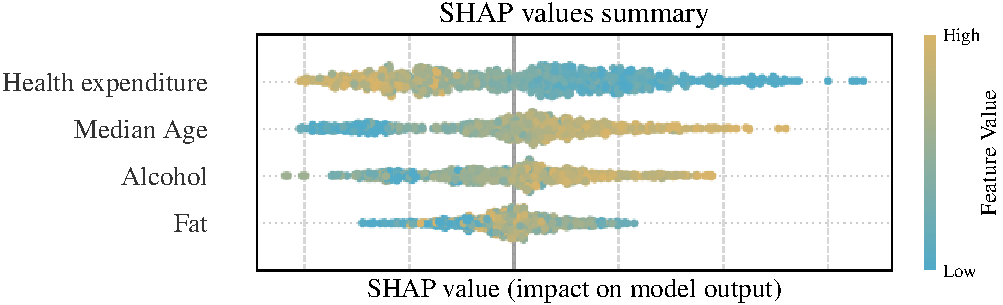
\includegraphics[width=\columnwidth]{fig/shap_values_summary.pdf}}
    \caption{Summary of SHAP values for a predictive model of disease death rate. 
    Each dot's color represents the feature's value (red high, blue low), and its position represents the impact on the model's output.
    The impact is measured by the SHAP value, which represents the feature's contribution to a change in the model's output.}
    \label{shap_values}
    \end{center}
    \vskip -0.2in
\end{figure}

To model the death rate of ischemic heart disease we tried using a linear model with different transformations of the data, but the results were not satisfactory.
Because of this, we decided to use random forest regression. 
We used the \texttt{RandomForestRegressor} from the \texttt{scikit-learn} library \citep{scikit-learn} with grid search to find the best parameters. Our best model had the 
$R^2$ score of $\approx0.82$ on the test set, while the $R^2$ score of the linear model was $\approx0.39$. The value represents the proportion of the variance that 
is explained by the model. We interpret the model using the SHAP (SHapley Additive exPlanations) values \citep{NIPS2017_7062} (see Figure \ref{shap_values}). SHAP values 
show how the impact of a feature on the model's output. The color gradient from pink to blue indicates the feature's value from low to high, 
showing how each feature contributes differently based on its value.

\begin{figure*}[ht]
    \vskip 0.2in
    \centering
    \centerline{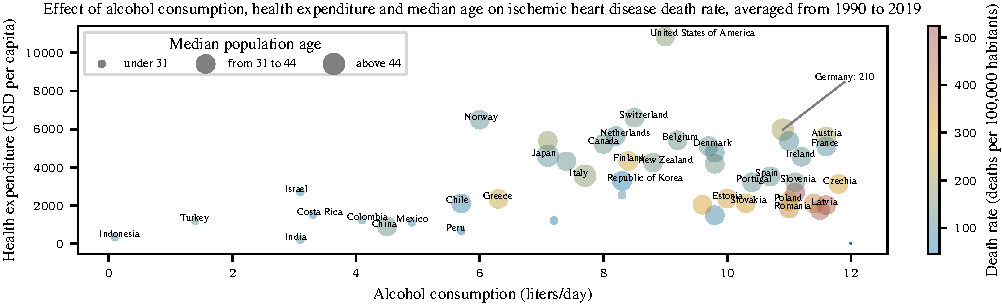
\includegraphics[]{fig/fig_bubble_plot_factors.pdf}}
    \caption{The combined effect of healthcare spending, alcohol consumption, and median age on the death rate of ischemic heart disease. Special 
        emphasis to the comparison between Germany, high income countries, and the world.}
    \label{bubble_plot_factors}
\end{figure*}

We can see that the effect of fat consumption is mixed and not very easy to interpret. The effect of the other three features 
(Healthcare spending, alcohol consumption, and median age) is more clear. For that reason, we decided to use only those three features in our final plot 
(see Figure \ref{bubble_plot_factors}) in which we show the combined effect of the three features on the death rate. The median age is divided into three groups, under 19, 19-38, and over 38. The size of the bubble represents the age group. The position of the bubble represents the healthcare spending and the alcohol consumption. The color represents the death rate from IHDs.
Counries with higher alcohol consumption (on the right) appear to have higher death rates.
It is clear that Germany is among the highest investors in healthcare, but it is also among the countries with the highest alcohol consumption. The median age is in the third group.



\section{Discussion \& Conclusion}\label{sec:conclusion}
% Use this section to briefly summarize the entire text. 
% Highlight limitations and problems, but also make clear statements where they are possible and supported by the analysis. 

In this project, we analyzed cardiovascular diseases with a specific focus on Germany.
We showed that the incidence rate of cardiovascular diseases in Germany is statistically significantly higher than the world average.
We analyzed some of the possible factors that could influence the death rate of ischemic heart disease, which is the most common cardiovascular disease in Germany.
Our model showed that the death rate of ischemic heart disease is influenced by healthcare spending, alcohol consumption, and median age, while 
the effect of fat consumption is mixed and not clear for interpretation. The fact that the effect of fat consumption is not clear is surprising, since it is 
a well-known risk factor for cardiovascular diseases.
We found that lower median age, lower alcohol consumption, and higher healthcare spending
all lead to lower death rates, which was to be expected.
Taking into account Germany's high healthcare spending and acceptable death to incidence ratio for cardiovascular diseases, we do not believe there to be an issue in the German health care system in comparison to the world.
We also found that the German alcohol consumption is higher than the world average (nearly three times as high as the world average), 
which could be a reason for the higher death rate.
The limitation of our analysis is that we didn't analyze all the possible factors that could influence the death rate of ischemic heart disease. 
Such factors could be smoking, vegetable consumption, or physical activity. We focused only on cardiovascular diseases, but it would be interesting to analyze less prevalent diseases as well.
Another possible extension of this project would be to explore if there is any genetic predisposition for cardiovascular diseases in Germany, using a genome-wide association study (GWAS).

\section*{Contribution Statement}
% Explain here, in one sentence per person, what each group member contributed. 
% For example, you could write: Max Mustermann collected and prepared data. Gabi Musterfrau and John Doe performed the data analysis. 
% Jane Doe produced visualizations. All authors will jointly wrote the text of the report. 
% Note that you, as a group, a collectively responsible for the report. Your contributions should be roughly equal in amount and difficulty.
This project was done in a group of three. Because of the amount of different data sources, there is no clear division of work. All of 
us worked on the data collection and analysis. Building on that work, each of us also produced visualizations for their part of the analysis.
Writing the report was a joint effort.

\bibliography{bibliography}
\bibliographystyle{icml2023}

\end{document}


% This document was modified from the file originally made available by
% Pat Langley and Andrea Danyluk for ICML-2K. This version was created
% by Iain Murray in 2018, and modified by Alexandre Bouchard in
% 2019 and 2021 and by Csaba Szepesvari, Gang Niu and Sivan Sabato in 2022.
% Modified again in 2023 by Sivan Sabato and Jonathan Scarlett.
% Previous contributors include Dan Roy, Lise Getoor and Tobias
% Scheffer, which was slightly modified from the 2010 version by
% Thorsten Joachims & Johannes Fuernkranz, slightly modified from the
% 2009 version by Kiri Wagstaff and Sam Roweis's 2008 version, which is
% slightly modified from Prasad Tadepalli's 2007 version which is a
% lightly changed version of the previous year's version by Andrew
% Moore, which was in turn edited from those of Kristian Kersting and
% Codrina Lauth. Alex Smola contributed to the algorithmic style files.
